% Dossier technique et de référence · la butée · version Bachelor (tronc commun)
% Compilation : xelatex (deux passes)
\documentclass[11pt,a4paper]{article}
\usepackage{fontspec}
\usepackage{polyglossia}
\setdefaultlanguage{french}
\providecommand{\og}{«~}\providecommand{\fg}{~»}
\usepackage[a4paper,margin=2.1cm,headheight=16pt,includehead,includefoot]{geometry}
\usepackage{amsmath,amssymb}
\usepackage{graphicx}
\usepackage{booktabs,array,tabularx,multirow}
\usepackage{xcolor}
\usepackage[most]{tcolorbox}
\usepackage{enumitem}
\usepackage{fancyhdr}
\usepackage{titlesec}
\usepackage{tikz}
\usepackage{pgfplots}
\pgfplotsset{compat=1.18}
\usetikzlibrary{arrows.meta,positioning,shapes.geometric,calc,patterns}
\usepackage[locale=FR,group-four-digits=true]{siunitx}
\usepackage{caption}
\usepackage[hidelinks,pdftitle={Dossier technique et de référence · la butée · Bachelor},pdfauthor={S. Jaubert}]{hyperref}

\definecolor{bleu}{HTML}{1F5C7A}
\definecolor{bleuclair}{HTML}{E8F1F6}
\definecolor{orange}{HTML}{C55A11}
\definecolor{orangeclair}{HTML}{FDF0E6}
\definecolor{gris}{HTML}{5F6B73}
\definecolor{grisclair}{HTML}{F2F4F5}
\definecolor{rouge}{HTML}{C62828}

\captionsetup{font=small,labelfont={bf,color=bleu},labelsep=colon}
\renewcommand{\figurename}{Fig.}
\renewcommand{\tablename}{Tab.}

\titleformat{\section}{\Large\bfseries\color{bleu}}{\thesection}{0.6em}{}
\titleformat{\subsection}{\large\bfseries\color{bleu}}{\thesubsection}{0.6em}{}
\titleformat{\subsubsection}{\normalsize\bfseries\color{bleu}}{\thesubsubsection}{0.6em}{}
\renewcommand{\thesection}{\Alph{section}}
\setlength{\parindent}{0pt}
\setlength{\parskip}{0.55em}

\newtcolorbox{retenir}[1][À retenir]{colback=bleuclair,colframe=bleu,fonttitle=\bfseries\small,title={#1},boxrule=0.6pt,arc=1pt,left=6pt,right=6pt,top=4pt,bottom=4pt}
\newtcolorbox{attention}[1][Attention]{colback=orangeclair,colframe=orange,fonttitle=\bfseries\small,title={#1},boxrule=0.6pt,arc=1pt,left=6pt,right=6pt,top=4pt,bottom=4pt}
\newtcolorbox{note}[1][Pour aller plus loin]{colback=grisclair,colframe=gris,fonttitle=\bfseries\small,title={#1},boxrule=0.6pt,arc=1pt,left=6pt,right=6pt,top=4pt,bottom=4pt,fontupper=\small}

\newcommand{\xbb}{\bar{\bar{X}}}
\newcommand{\Rb}{\bar{R}}
\newcommand{\diameter}{\varnothing}
\setlength{\emergencystretch}{2.5em}
\newcommand{\cote}{\diameter\,12^{\,0}_{-0{,}15}}
\newcommand{\xl}[1]{\texttt{\small #1}}

\pagestyle{fancy}
\fancyhf{}
\fancyhead[L]{\raisebox{-0.25\height}{
\includegraphics[height=12pt]{logo.png}}\ \small\color{bleu}Dossier technique et de référence \textperiodcentered\ la butée}
\fancyhead[R]{\small\color{bleu}\leftmark}
\fancyfoot[L]{\scriptsize\color{gris}Capabilité et SPC \textperiodcentered\ Bachelor}
\fancyfoot[C]{\small\thepage}
\fancyfoot[R]{\scriptsize\color{gris}Pôle Formation UIMM CVDL \textperiodcentered\ S. Jaubert \textperiodcentered\ novembre 2026}
\renewcommand{\headrulewidth}{0.4pt}
\renewcommand{\sectionmark}[1]{\markboth{\thesection. #1}{}}

\begin{document}

%======================== COUVERTURE ========================
\begin{titlepage}
\centering
\vspace*{1.2cm}

\includegraphics[height=2.6cm]{logo.png}\par
\vspace{1.6cm}
{\large\color{gris}Capabilité et SPC \textperiodcentered\ Bachelor, tronc commun\par}
\vspace{0.8cm}
{\fontsize{26}{32}\selectfont\color{bleu}Dossier technique\\[2pt] et de référence\par}
\vspace{0.6cm}
{\Large\color{bleu}La butée : diamètre du téton $\cote$\par}
\vspace{1.1cm}
\begin{tikzpicture}[scale=0.5]
\fill[grisclair] (0,-1.6) rectangle (3.6,1.6); \draw[thick] (0,-1.6) rectangle (3.6,1.6);
\fill[grisclair] (3.6,-1) rectangle (7,1); \draw[thick] (3.6,-1) -- (6.8,-1) -- (7,-0.8) -- (7,0.8) -- (6.8,1) -- (3.6,1);
\draw[dash dot,gris] (-0.6,0) -- (7.6,0);
\end{tikzpicture}
\par\vspace{1.2cm}
\begin{minipage}{0.78\textwidth}
\rule{\linewidth}{0.6pt}\par\small
Partie A. Le dossier technique : la pièce, le dessin, la matière, les instruments, les données, la traçabilité.\par
Partie B. Comprendre et lire une carte de contrôle : la synthèse.\par
Partie C. La référence : toutes les formules utilisées dans la formation, avec leur incertitude.\par
Partie D. Les tables de coefficients.\par
Partie E. Les sources.\par
\rule{\linewidth}{0.6pt}
\end{minipage}
\vfill
{\small Pôle Formation UIMM Centre-Val de Loire \textperiodcentered\ S. Jaubert \textperiodcentered\ novembre 2026\par}
{\footnotesize Document de référence remis à chaque étudiant. À garder avec le livret de TP.\par}
{\scriptsize\color{gris} Version Bachelor du dossier BTS ATI : parties A à E reprises, étude R\&R, intervalles de confiance, test d'Anderson-Darling, efficacité des cartes et surdispersion ajoutés.\par}
\end{titlepage}

%======================== MODE D'EMPLOI ========================
\setcounter{page}{1}
\markboth{Mode d'emploi}{}
\section*{Mode d'emploi}
Ce dossier accompagne le livret de TP. Le livret dit ce qu'on fait. Le dossier dit sur quoi on s'appuie : la pièce, ses exigences, les formules, leurs hypothèses et leurs sources. Il reste valable après les TP, sur une autre cote, dans votre entreprise.

Par rapport à la version BTS, ce dossier ajoute ce qu'un technicien de niveau Bachelor doit savoir défendre devant un client ou un auditeur : la part de la mesure dans la variation (étude R\&R), l'incertitude des indices calculés sur peu de valeurs, un vrai test de normalité, ce qu'une carte détecte et en combien de temps, et ce qu'il faut faire quand le modèle d'une carte aux attributs ne tient pas.

\begin{center}\small
\begin{tabularx}{\textwidth}{@{}Xll@{}}
\toprule
\textbf{Vous cherchez} & \textbf{Où regarder} & \textbf{Page}\\\midrule
La cote, la tolérance, la matière & A.2 Dessin, A.3 Matière & \pageref{sec:dessin}\\
Quel instrument, quelle résolution & A.4 Instruments & \pageref{sec:instr}\\
D'où vient la justesse d'un micromètre & A.7 Traçabilité & \pageref{sec:traca}\\
Ce que montre une carte, comment la lire & B. Comprendre et lire une carte & \pageref{sec:B}\\
Que faire quand la carte sonne & B.6 Réagir à une alarme & \pageref{sec:reagir}\\
Intervalle de confiance d'une moyenne, d'un écart-type & C.2 Estimation & \pageref{sec:ic}\\
Henry, Anderson-Darling & C.3 Normalité & \pageref{sec:normalite}\\
Cg, Cgk & C.4 Capabilité de l'instrument & \pageref{sec:cg}\\
\%R\&R, ndc, ANOVA de mesure & C.5 Étude R\&R & \pageref{sec:rr}\\
Cp, Cpk, Pp, Ppk et leur incertitude & C.6 Capabilité du procédé & \pageref{sec:cap}\\
Les limites d'une carte $\bar X$/R & C.7 Cartes $\bar X$/R & \pageref{sec:xbarr}\\
XmR, cartes aux attributs, carte p$'$ & C.9 et C.10 & \pageref{sec:xmr}\\
Risque de fausse alarme, ARL & C.11 Efficacité d'une carte & \pageref{sec:arl}\\
Un coefficient ($d_2$, $A_2$, $K_1$, $D'_{s2}$\ldots) & D. Tables & \pageref{sec:D}\\
D'où vient une formule & E. Sources & \pageref{sec:E}\\
\bottomrule
\end{tabularx}
\end{center}

\textbf{Correspondance avec le livret de TP.} TP 1 (le système de mesure) : A.4, A.5, A.7, C.4, C.5 et D. TP 2 (le lot) : A.1 à A.3, A.6, C.1 à C.3. TP 3 (la capabilité) : C.6, avec C.5 pour la part de la mesure. TP 4 (la carte $\bar X$/R) : B, C.7, C.11 et D. TP 5 (choisir sa carte) : B.8, C.9 et C.10.

\textbf{Conventions.} Les décimales s'écrivent avec une virgule. Les dimensions sont en millimètres. Les références entre crochets, par exemple [1], renvoient à la liste des sources (partie E). Une affirmation sans référence est soit une définition, soit un calcul refait et vérifié pour ce dossier. Les noms de fonctions Excel sont ceux de la version française.

{\small\tableofcontents}

\clearpage
%======================== A ========================
\section{Le dossier technique}
\subsection{Le cas d'étude}
Un sous-traitant produit des butées en série renouvelable, \num{1500} pièces par mois. La pièce est tournée : chariotage et dressage. La caractéristique suivie est le diamètre du téton. Le contrôle se fait à côté du poste de tournage. Le contrôleur prélève, à intervalles réguliers, un échantillon de 5 pièces consécutives.

\begin{retenir}[{Ce cas est un cas pédagogique}]
L'entreprise, la cadence et l'historique des échantillons 1 à 6 viennent d'un ancien travail pratique du Pôle Formation. Les butées, elles, sont réelles : vous les avez dans les mains. Les échantillons 7 à 10, ce sont vos mesures. La butée sert de fil rouge aux trois parcours du Bachelor : la même démarche vaut pour une position de préhension robot, un couple de serrage ou un alésage de palier remis en état.
\end{retenir}

\subsection{Dessin de définition}\label{sec:dessin}
\begin{figure}[h]
\centering
\begin{tikzpicture}[scale=1.15,>=Latex]
\fill[grisclair] (0,-1.9) rectangle (4.2,1.9); \draw[thick] (0,-1.9) rectangle (4.2,1.9);
\fill[grisclair] (4.2,-1.25) -- (8.1,-1.25) -- (8.35,-1.0) -- (8.35,1.0) -- (8.1,1.25) -- (4.2,1.25) -- cycle;
\draw[thick] (4.2,-1.25) -- (8.1,-1.25) -- (8.35,-1.0) -- (8.35,1.0) -- (8.1,1.25) -- (4.2,1.25);
\draw[dash dot,gris] (-0.7,0) -- (9.0,0);
\node[gris,font=\small] at (2.1,0.35) {collerette};
\node[gris,font=\small] at (6.6,-1.6) {téton};
% cotes
\draw[thin] (0,1.9) -- (0,2.75); \draw[thin] (8.35,1.0) -- (8.35,2.75);
\draw[<->] (0,2.6) -- node[above,font=\small]{$30\pm0{,}5$} (8.35,2.6);
\draw[thin] (0,-1.9) -- (0,-2.75); \draw[thin] (4.2,-1.9) -- (4.2,-2.75);
\draw[<->] (0,-2.6) -- node[below,font=\small]{$15\pm0{,}1$} (4.2,-2.6);
\draw[thin,rouge] (8.35,1.0) -- (9.1,1.25); \draw[thin,rouge] (8.35,-1.0) -- (9.1,-1.25);
\draw[<->,rouge,thick] (9.0,-1.25) -- node[right,font=\small]{$\cote$} (9.0,1.25);
\end{tikzpicture}
\caption{Dessin de définition de la butée, redessiné d'après le dessin d'origine. Proportions indicatives. En rouge, la caractéristique suivie.}
\end{figure}

\begin{center}\small
\begin{tabular}{@{}ll@{}}
\toprule
\textbf{Élément} & \textbf{Valeur}\\\midrule
Caractéristique suivie & diamètre du téton, $\cote$\\
Tolérance inférieure, supérieure & $T_I = 11{,}85$ ; $T_S = 12{,}00$\\
Intervalle de tolérance & $IT = T_S - T_I = 0{,}15$\\
Milieu de la tolérance & $(T_I+T_S)/2 = 11{,}925$\\
Longueur totale & $30\pm0{,}5$\\
Longueur de la collerette & $15\pm0{,}1$\\
Non cotés sur le dessin d'origine & diamètre de la collerette, chanfrein du téton\\
Matière & AU4G (voir A.3)\\\bottomrule
\end{tabular}
\end{center}

\begin{retenir}[{Une cote $\cote$ se lit ainsi}]
Cote nominale 12, écart supérieur 0, écart inférieur $-0{,}15$. Toute pièce entre 11,85 et 12,00 inclus est conforme. Le milieu de la tolérance n'est pas 12 mais 11,925 : c'est là qu'un procédé bien réglé devrait centrer sa production.
\end{retenir}

\subsection{Matière}
AU4G est l'ancienne désignation française d'un alliage d'aluminium au cuivre. Sa désignation européenne est EN AW-2017A, symbole chimique AlCu4MgSi(A) [11]. C'est un alliage courant pour l'usinage. Ne pas le confondre avec l'alliage 2024, dont l'ancienne désignation française est AU4G1 [11].

\subsection{Les instruments de la formation}\label{sec:instr}
\begin{center}\small
\begin{tabular}{@{}lccc@{}}
\toprule
\textbf{Instrument} & \textbf{Résolution} & \textbf{Résolution / IT} & \textbf{Règle des dix}\\\midrule
Pied à coulisse au 1/50 (6 instruments) & 0,02 mm & 13,3 \% & non respectée\\
Micromètre numérique 0-25 mm, M1 à M6 & 0,001 mm & 0,7 \% & respectée\\\bottomrule
\end{tabular}
\end{center}

\textbf{Règle des dix.} La résolution de l'instrument doit diviser la tolérance en au moins dix parties [8]. Pour le téton : $IT/10 = 0{,}015$ mm. Le pied à coulisse au 1/50 ne la respecte pas. La limite 11,85 n'est même pas lisible : il lit 11,84 ou 11,86. La méthode de capabilité de l'instrument (C.4) est plus exigeante : résolution au plus 5 \% de la tolérance [7], soit 0,0075 mm ici.

\textbf{Ce que la résolution coûte.} Lire avec un pas $q$ revient à ajouter une erreur d'arrondi répartie uniformément sur $[-q/2\,;\,q/2]$. Son écart-type vaut $q/\sqrt{12}$ : 0,0058 mm pour le pied au 1/50, 0,0003 mm pour le micromètre. La résolution n'est qu'une borne basse de l'erreur de mesure : l'étude R\&R (C.5) mesure le reste.

\textbf{Mode opératoire de mesure.} Petit diamètre du téton, au trait repère, en tenant la pièce toujours de la même façon. Au micromètre, fermer avec le cliquet, jamais avec le tambour. Noter les trois décimales affichées.

\subsection{Les butées de la formation}\label{sec:butees}
\begin{minipage}[t]{0.58\textwidth}
\vspace{0pt}
Vingt butées réelles, numérotées de 1 à 20. Le numéro tient lieu d'ordre de fabrication. Elles forment les échantillons 7 à 10 :

\begin{center}\small
\begin{tabular}{@{}cc@{}}\toprule
\textbf{Échantillon} & \textbf{Butées}\\\midrule
7 & 1 à 5\\ 8 & 6 à 10\\ 9 & 11 à 15\\ 10 & 16 à 20\\\bottomrule
\end{tabular}
\end{center}
Trois butées de référence, repérées par une pastille rouge, servent à l'étude de type 1 : R1 = butée n° 8, R2 = n° 14, R3 = n° 15. L'étude R\&R du TP 1 utilise les butées n° 1 à 10.
\end{minipage}\hfill
\begin{minipage}[t]{0.38\textwidth}
\vspace{0pt}\centering
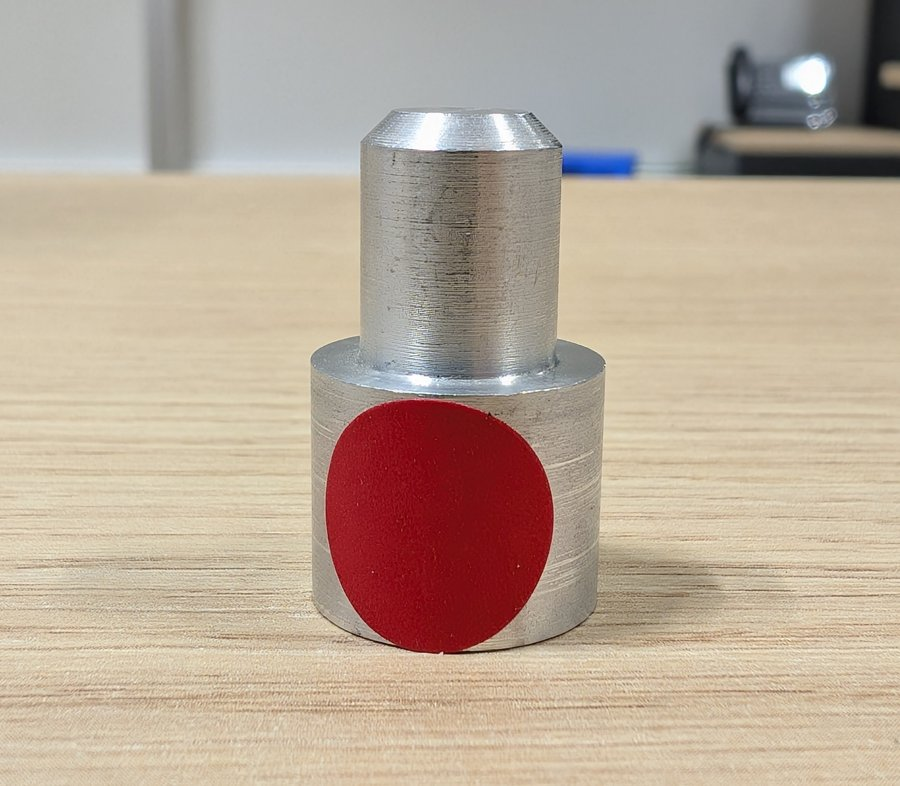
\includegraphics[width=\linewidth]{butee.png}\par
{\small Butée de référence (pastille rouge).}
\end{minipage}

\subsection{Les données}\label{sec:donnees}
Dossier \xl{Donnees} : un fichier .csv par activité, séparateur point-virgule, décimale virgule.

\begin{center}\small
\begin{tabularx}{\textwidth}{@{}lX@{}}
\toprule
\textbf{Fichier} & \textbf{Contenu}\\\midrule
\xl{Cg\_releve\_butee\_reference.csv} & grille vide, 25 essais : étude de type 1 (TP 1)\\
\xl{RR\_releve\_butees.csv} & grille vide, 2 opérateurs $\times$ 3 essais $\times$ 10 butées : étude R\&R (TP 1)\\
\xl{Butees\_diametre.csv} & échantillons 1 à 6 (30 valeurs au 0,01 mm, historique fourni) ; lignes 7 à 10 vides, pour vos mesures au 0,001 mm (TP 2 à 4)\\
\xl{Butees\_diametre\_colonne.csv} & les mêmes 30 valeurs en une colonne, pour un logiciel de statistique\\
\xl{SPC-1}, \xl{SPC-3}, \xl{SPC-16} & inspection par lots, liquide par lots, sur-réglage (TP 5)\\
\xl{SPC-2}, \xl{SPC-8}, \xl{SPC-10} & pression, billes, dimension usinée (annexe B du livret)\\\bottomrule
\end{tabularx}
\end{center}

\begin{attention}[{Deux résolutions dans un même fichier}]
Les échantillons 1 à 6 ont été arrondis au centième. Les vôtres sont au millième. Ce mélange se voit sur un histogramme, sur la carte des étendues, et il fausse les tests de normalité (C.3). Il faut le savoir avant d'interpréter. Dix échantillons, c'est aussi peu : les limites calculées sont provisoires (C.7) et les indices de capabilité sont imprécis (C.6).
\end{attention}

\subsection{La traçabilité : du mètre au micromètre}\label{sec:traca}
Un micromètre est juste parce qu'on l'a comparé à quelque chose de plus juste que lui. La \emph{traçabilité métrologique} est la propriété d'un résultat de mesure relié à une référence par une chaîne ininterrompue et documentée d'étalonnages, chacun ajoutant sa part d'incertitude.

\begin{figure}[h]
\centering
\begin{tikzpicture}[node distance=4mm and 3mm, box/.style={draw=bleu,fill=bleuclair,rounded corners=1pt,align=center,font=\footnotesize,minimum height=12mm,text width=24mm}, >=Latex]
\node[box] (a) {Définition du mètre\\(SI, BIPM)};
\node[box,right=of a] (b) {Laser étalon\\laboratoire national};
\node[box,right=of b] (c) {Cales étalons\\laboratoire accrédité};
\node[box,right=of c] (d) {Cales de l'atelier,\\bague étalon};
\node[box,right=of d] (e) {Micromètre\\M1 à M6};
\draw[->,thick,bleu] (a)--(b); \draw[->,thick,bleu] (b)--(c); \draw[->,thick,bleu] (c)--(d); \draw[->,thick,bleu] (d)--(e);
\node[below=2mm of c,font=\footnotesize,gris] {incertitude croissante de gauche à droite};
\end{tikzpicture}
\caption{Une chaîne de traçabilité, schéma de principe. Les maillons réels dépendent de l'entreprise et de ses prestataires.}
\end{figure}

Depuis 1983, le mètre est la longueur du trajet parcouru dans le vide par la lumière pendant $1/\num{299792458}$ de seconde. Depuis la révision du SI de 2019, cette définition s'écrit en fixant la valeur exacte de la vitesse de la lumière, $c = \num{299792458}$ m/s, et de la fréquence hyperfine du césium 133, $\Delta\nu_{\mathrm{Cs}} = \num{9192631770}$ Hz, qui définit la seconde [26]. L'histoire de cette définition, de la méridienne de Delambre et Méchain au césium, est racontée dans la synthèse remise avec le kit [25].

\begin{retenir}[{Trois études, trois questions}]
\textbf{Étalonnage} : l'instrument donne-t-il la bonne valeur sur un étalon ? Il se fait en laboratoire, il est relié à la chaîne ci-dessus. \textbf{Étude de type 1 (Cg, Cgk)} : au poste, sur une pièce de référence, l'instrument est-il assez fidèle et assez juste pour cette tolérance ? \textbf{Étude R\&R} : avec de vraies pièces et de vrais opérateurs, quelle part de la variation observée vient de la mesure ? Aucune des trois ne remplace les deux autres.
\end{retenir}

\clearpage
%======================== B ========================
\section{Comprendre et lire une carte de contrôle}\label{sec:B}
\subsection{Pourquoi une carte}
Deux pièces ne sont jamais identiques. Shewhart distingue deux familles de causes de variation [12] :
\begin{itemize}[nosep]
\item les \textbf{causes communes} : nombreuses, petites, toujours présentes (jeu machine, température, matière). Elles forment le bruit de fond du procédé. On ne les supprime pas en réglant : on les réduit en changeant le procédé ;
\item les \textbf{causes spéciales} : rares, identifiables, ponctuelles (outil cassé, mauvais réglage, nouveau lot de matière). Elles doivent être trouvées et éliminées.
\end{itemize}
Une carte de contrôle sert à une seule chose : dire, à chaque prélèvement, si une cause spéciale est probablement apparue. Si oui, on agit. Si non, on ne touche à rien. Le mot \og probablement \fg{} compte : une carte est un test statistique répété, avec ses deux risques (C.11).

\begin{retenir}
Un procédé \og sous contrôle \fg{} n'est pas un procédé \og bon \fg. Il est stable et prévisible. Il peut être stable et produire des pièces hors tolérance : c'est alors un problème de capabilité (C.6), pas de réglage.
\end{retenir}

\subsection{Voix du client, voix du procédé}
Les \textbf{tolérances} sont fixées par le client sur le dessin. Elles portent sur chaque pièce. Les \textbf{limites de contrôle} sont calculées à partir du procédé lui-même. Sur une carte $\bar X$, elles portent sur des moyennes d'échantillons, qui varient moins que les pièces : l'écart-type d'une moyenne de $n$ pièces indépendantes vaut $\sigma/\sqrt n$.

\begin{figure}[h]
\centering
\begin{tikzpicture}
\begin{axis}[width=13cm,height=5.2cm,axis lines=left,ytick=\empty,xtick={-4.5,-1.342,1.342,4.5},xticklabels={$T_I$,LCI,LCS,$T_S$},xmin=-5.2,xmax=5.2,ymin=0,ymax=0.95,xlabel={valeur mesurée},xlabel style={font=\small},samples=200,domain=-5:5,clip=false]
\addplot[gris,thick] {exp(-x^2/2)/sqrt(2*pi)};
\addplot[bleu,thick,fill=bleuclair,fill opacity=0.6] {exp(-x^2*5/2)*sqrt(5)/sqrt(2*pi)};
\draw[rouge,thick] (axis cs:-4.5,0) -- (axis cs:-4.5,0.9); \draw[rouge,thick] (axis cs:4.5,0) -- (axis cs:4.5,0.9);
\draw[bleu,thick,dashed] (axis cs:-1.342,0) -- (axis cs:-1.342,0.9); \draw[bleu,thick,dashed] (axis cs:1.342,0) -- (axis cs:1.342,0.9);
\node[font=\footnotesize,bleu] at (axis cs:2.35,0.62) {moyennes de 5 pièces : $\sigma/\sqrt5$};
\node[font=\footnotesize,gris] at (axis cs:2.6,0.22) {pièces : $\sigma$};
\node[font=\footnotesize,rouge,above] at (axis cs:4.5,0.9) {client};
\node[font=\footnotesize,bleu,above] at (axis cs:0,0.9) {procédé};
\end{axis}
\end{tikzpicture}
\caption{Les tolérances (rouge) jugent chaque pièce. Les limites de contrôle (bleu) jugent la moyenne d'un échantillon. Exemple schématique : limites à 3 sigmas, $n=5$.}
\end{figure}

\begin{attention}[{L'erreur la plus fréquente}]
Tracer les tolérances sur une carte $\bar X$, ou calculer les limites à partir des tolérances. Les deux n'ont rien à voir. Une moyenne peut être dans les limites de contrôle alors qu'une pièce de l'échantillon est hors tolérance.
\end{attention}

\subsection{Anatomie d'une carte \texorpdfstring{$\bar X$}{X}/R}
Une carte $\bar X$/R, ce sont deux graphiques l'un sous l'autre, avec le même axe horizontal : le numéro de l'échantillon, dans l'ordre de prélèvement.

\begin{figure}[h]
\centering
\begin{tikzpicture}
\begin{axis}[width=13cm,height=5cm,xmin=0.5,xmax=20.5,ymin=-3.8,ymax=3.8,ytick={-3.09,-1.96,0,1.96,3.09},yticklabels={LCI,LSI,LC,LSS,LCS},xtick={1,5,10,15,20},xlabel={n° d'échantillon},xlabel style={font=\small},tick label style={font=\footnotesize}]
\fill[orangeclair] (axis cs:0.5,1.96) rectangle (axis cs:20.5,3.09); \fill[orangeclair] (axis cs:0.5,-1.96) rectangle (axis cs:20.5,-3.09);
\addplot[rouge,thick,domain=0.5:20.5] {3.09}; \addplot[rouge,thick,domain=0.5:20.5] {-3.09};
\addplot[orange,dashed,domain=0.5:20.5] {1.96}; \addplot[orange,dashed,domain=0.5:20.5] {-1.96};
\addplot[black,domain=0.5:20.5] {0};
\addplot[bleu,thick,mark=*,mark size=1.4pt] table[x=i,y=x] {fig/alarme0.dat};
\end{axis}
\end{tikzpicture}
\caption{Carte des moyennes, limites AFNOR, en écarts-types de la moyenne. Procédé sous contrôle : les points se répartissent au hasard autour de la ligne centrale. Données simulées (loi normale, graine fixée).}
\end{figure}

\begin{center}\small
\begin{tabularx}{\textwidth}{@{}lX@{}}\toprule
\textbf{Élément} & \textbf{Rôle}\\\midrule
Ligne centrale & la moyenne des moyennes $\xbb$ (carte $\bar X$), l'étendue moyenne $\Rb$ (carte R)\\
LCS, LCI & limites de contrôle supérieure et inférieure. Un point au-delà : on agit\\
LSS, LSI & limites de surveillance (convention AFNOR seulement). Un point entre surveillance et contrôle : on refait un prélèvement\\
Carte R & surveille la dispersion à l'intérieur de chaque échantillon\\
Carte $\bar X$ & surveille la position (le réglage) du procédé\\\bottomrule
\end{tabularx}
\end{center}

\subsection{Deux conventions de limites}
\begin{center}\small
\begin{tabularx}{\textwidth}{@{}lXX@{}}\toprule
 & \textbf{AFNOR (tradition française)} & \textbf{Shewhart (3 sigmas)}\\\midrule
Limites de contrôle & $\pm3{,}09$ écarts-types : 1 chance sur \num{1000} de chaque côté de sortir sans cause spéciale & $\pm3$ écarts-types : environ 1,35 chance sur \num{1000} de chaque côté\\
Limites de surveillance & $\pm1{,}96$ écart-type : 2,5 \% de chaque côté & pas de limite de surveillance dans la règle de base\\
Carte R & limites tirées de la loi exacte de l'étendue & limites $D_3\Rb$ et $D_4\Rb$, approximation à 3 écarts-types\\
Où on la trouve & manuels et entreprises françaises [2] & ISO 7870-2, AIAG, la plupart des logiciels [3][5]\\\bottomrule
\end{tabularx}
\end{center}
Les deux conventions donnent des limites très proches pour la carte $\bar X$. Elles diffèrent davantage sur la carte R. L'important est d'écrire la convention choisie sur la carte et de s'y tenir. Sur l'efficacité de chacune, voir C.11.

\subsection{Lire une carte en quatre temps}
\begin{enumerate}[nosep]
\item \textbf{La carte R d'abord.} Si la dispersion n'est pas stable, les limites de la carte $\bar X$, qui en dépendent, ne veulent rien dire.
\item \textbf{La carte $\bar X$ ensuite}, point par point, dans l'ordre chronologique.
\item \textbf{Les règles d'alarme} (ci-dessous) : un point isolé, puis les séries.
\item \textbf{La décision} : ne rien faire, refaire un prélèvement, ou arrêter et chercher. Écrire ce qu'on a fait sur la carte.
\end{enumerate}

\subsubsection*{Les règles d'alarme retenues pour la formation}\label{sec:regles}
\begin{center}\small
\begin{tabularx}{\textwidth}{@{}cXX@{}}\toprule
 & \textbf{Ce qu'on voit} & \textbf{Ce que ça veut probablement dire}\\\midrule
1 & 1 point hors des limites de contrôle & une cause spéciale vient d'apparaître\\
2 & 7 points de suite du même côté de la ligne centrale & le réglage a bougé\\
3 & 6 points de suite qui montent, ou qui descendent & une dérive : usure d'outil, échauffement\\
4 & cartes AFNOR : 1 point entre surveillance et contrôle & doute : refaire un prélèvement tout de suite\\
5 & 1 point hors limites sur la carte R & la dispersion a changé : outil, matière, bridage, mesure\\\bottomrule
\end{tabularx}
\end{center}

\begin{note}[{D'où viennent ces règles, et ce qu'elles coûtent}]
La règle 1 est la règle de base de Shewhart [12]. Les règles de séries sont des tests de configuration. La liste la plus citée compte huit tests [13] ; les logiciels l'utilisent souvent, avec 9 points du même côté au lieu de 7, et 6 points montants ou descendants. La règle des 7 points est un usage répandu en France. Chaque règle ajoutée détecte plus tôt, mais sonne aussi plus souvent à tort. Avec la seule règle 1 (3 sigmas), un procédé stable donne en moyenne une fausse alarme tous les 370 échantillons. Avec les règles 1 et 2, tous les 95 environ ; avec les règles 1, 2 et 3, tous les 80 environ (simulation, C.11). Dans votre entreprise, c'est la règle écrite au poste qui s'applique : vérifiez-la.
\end{note}

\subsection{Réagir à une alarme}\label{sec:reagir}
Le \textbf{plan de réaction} dit, pour chaque alarme, qui fait quoi. Il est écrit avant, affiché au poste, et suivi pendant. En anglais, on parle d'OCAP (\emph{out of control action plan}). Il répond à cinq questions :
\begin{enumerate}[nosep]
\item \textbf{Arrêter ?} Qui décide d'arrêter la machine, et à partir de quelle alarme.
\item \textbf{Les pièces ?} Que fait-on des pièces produites depuis le dernier point correct : on les isole, on les trie, on les contrôle à 100 \%.
\item \textbf{Chercher.} Qui cherche la cause : outil, réglage, matière, bridage, instrument, opérateur. On valide la mesure avant de toucher la machine.
\item \textbf{Corriger.} Une action sur la cause, pas sur le symptôme.
\item \textbf{Tracer.} Écrire sur la carte, au point concerné : la cause trouvée et l'action menée. Une carte sans annotation ne sert pas à améliorer le procédé.
\end{enumerate}

\begin{figure}[h]
\centering
\pgfplotsset{mini/.style={width=7.6cm,height=3.7cm,xmin=0.5,xmax=20.5,ymin=-3.8,ymax=3.8,xtick={1,10,20},tick label style={font=\scriptsize},title style={font=\small\bfseries}}}
\begin{tikzpicture}
\begin{axis}[mini,title={Règle 1 : un point hors limites},ytick={-3.09,0,3.09},yticklabels={LCI,LC,LCS}]
\addplot[rouge,thick,domain=0.5:20.5]{3.09};\addplot[rouge,thick,domain=0.5:20.5]{-3.09};\addplot[black,domain=0.5:20.5]{0};
\addplot[bleu,thick,mark=*,mark size=1.2pt] table[x=i,y=x]{fig/alarme1.dat};
\draw[rouge,thick] (axis cs:10,3.5) circle[radius=4pt];
\end{axis}
\end{tikzpicture}\hfill
\begin{tikzpicture}
\begin{axis}[mini,title={Règle 2 : 7 points du même côté},ytick={-3.09,0,3.09},yticklabels={LCI,LC,LCS}]
\fill[orangeclair] (axis cs:11.5,-0.2) rectangle (axis cs:18.5,2.2);
\addplot[rouge,thick,domain=0.5:20.5]{3.09};\addplot[rouge,thick,domain=0.5:20.5]{-3.09};\addplot[black,domain=0.5:20.5]{0};
\addplot[bleu,thick,mark=*,mark size=1.2pt] table[x=i,y=x]{fig/alarme2.dat};
\end{axis}
\end{tikzpicture}\\[2mm]
\begin{tikzpicture}
\begin{axis}[mini,title={Règle 3 : 6 points qui montent},ytick={-3.09,0,3.09},yticklabels={LCI,LC,LCS}]
\fill[orangeclair] (axis cs:12.5,-1.4) rectangle (axis cs:18.5,1.9);
\addplot[rouge,thick,domain=0.5:20.5]{3.09};\addplot[rouge,thick,domain=0.5:20.5]{-3.09};\addplot[black,domain=0.5:20.5]{0};
\addplot[bleu,thick,mark=*,mark size=1.2pt] table[x=i,y=x]{fig/alarme3.dat};
\end{axis}
\end{tikzpicture}\hfill
\begin{tikzpicture}
\begin{axis}[mini,title={Règle 4 : zone de surveillance},ytick={-3.09,-1.96,0,1.96,3.09},yticklabels={LCI,LSI,LC,LSS,LCS}]
\addplot[rouge,thick,domain=0.5:20.5]{3.09};\addplot[rouge,thick,domain=0.5:20.5]{-3.09};\addplot[black,domain=0.5:20.5]{0};
\addplot[orange,dashed,domain=0.5:20.5]{1.96};\addplot[orange,dashed,domain=0.5:20.5]{-1.96};
\addplot[bleu,thick,mark=*,mark size=1.2pt] table[x=i,y=x]{fig/alarme4.dat};
\draw[orange,thick] (axis cs:14,2.4) circle[radius=4pt];
\end{axis}
\end{tikzpicture}
\caption{Les quatre alarmes de la carte $\bar X$. Données simulées (loi normale, graine fixée, motif ajouté), en écarts-types de la moyenne, limites AFNOR. Chaque carte a été vérifiée par programme : elle ne déclenche que la règle de son titre.}
\end{figure}

\begin{attention}[{Le sur-réglage}]
Corriger le réglage à chaque point qui s'écarte de la ligne centrale, sans alarme, augmente la dispersion au lieu de la réduire. C'est la leçon de l'entonnoir de Deming [14]. Dans le cas le plus simple (on corrige à chaque pièce de tout l'écart à la cible), la variance double : l'écart-type est multiplié par $\sqrt2 \approx 1{,}41$. Règle : on ne touche au procédé que sur alarme.
\end{attention}

\subsection{Erreurs fréquentes}
\begin{center}\small
\begin{tabularx}{\textwidth}{@{}XX@{}}\toprule
\textbf{Erreur} & \textbf{Correction}\\\midrule
Mettre les tolérances sur la carte $\bar X$ & tolérances pour les pièces, limites pour les moyennes (B.2)\\
Recalculer les limites à chaque nouveau point & limites calculées sur une période de référence stable (phase 1), puis figées (phase 2)\\
Calculer les limites sur une période avec des causes spéciales & écarter les échantillons expliqués, recalculer, vérifier\\
Lire la carte $\bar X$ sans regarder la carte R & carte R d'abord (B.5)\\
Régler à chaque point & réagir sur alarme seulement (B.6)\\
Confondre stable et capable & stable : la carte ; capable : Cp et Cpk (C.6)\\
Un instrument trop grossier ou des opérateurs qui mesurent différemment & résolution, étude de type 1, étude R\&R avant de juger le procédé (C.4, C.5)\\
Annoncer un Cpk sans dire sur combien de valeurs & donner la borne basse de confiance (C.6)\\\bottomrule
\end{tabularx}
\end{center}

\subsection{Choisir sa carte}
\begin{figure}[h]
\centering
\begin{tikzpicture}[>=Latex,font=\small,
 q/.style={draw=bleu,fill=bleuclair,rounded corners=2pt,align=center,minimum width=28mm,minimum height=9mm},
 r/.style={draw=orange,fill=orangeclair,rounded corners=2pt,align=center,minimum width=20mm,minimum height=8mm,font=\small\bfseries}]
\node[q] (top) at (0,0) {Que relève-t-on ?};
\node[q] (mes) at (-4,-1.6) {Une mesure\\(longueur, masse\ldots)};
\node[q] (cpt) at (4,-1.6) {Un comptage};
\node[q] (ech) at (-5.6,-3.4) {Échantillons\\de $n\ge2$ pièces};
\node[q] (une) at (-2.4,-3.4) {Une valeur\\à la fois};
\node[q] (nc) at (2.4,-3.4) {Pièces\\non conformes};
\node[q] (def) at (5.6,-3.4) {Défauts\\sur une pièce};
\node[r] (xr) at (-5.6,-5.1) {$\bar X$/R\\{\footnotesize\mdseries ($\bar X$/s si $n>10$)}};
\node[r] (xm) at (-2.4,-5.1) {XmR};
\node[r] (p) at (2.4,-5.1) {p ou np};
\node[r] (c) at (5.6,-5.1) {c ou u};
\foreach \a/\b in {top/mes,top/cpt,mes/ech,mes/une,cpt/nc,cpt/def,ech/xr,une/xm,nc/p,def/c} \draw[->,thick,gris] (\a)--(\b);
\end{tikzpicture}
\caption{Choisir la carte selon la donnée. np et c si l'effectif contrôlé est constant ; p et u s'il varie. Si la dispersion observée dépasse celle du modèle, voir la carte p$'$ (C.10).}
\end{figure}

\clearpage
%======================== C ========================
\section{La référence : les formules}
\subsection{Notations et statistiques de base}\label{sec:notations}
Un échantillon $i$ contient $n$ pièces, de valeurs $x_{i1},\dots,x_{in}$. On dispose de $k$ échantillons, soit $N=kn$ valeurs.

\begin{center}\small
\renewcommand{\arraystretch}{1.5}
\begin{tabularx}{\textwidth}{@{}Xll@{}}\toprule
\textbf{Grandeur} & \textbf{Formule} & \textbf{Excel}\\\midrule
Moyenne de l'échantillon $i$ & $\bar x_i=\frac1n\sum_{j=1}^n x_{ij}$ & \xl{MOYENNE}\\
Étendue de l'échantillon $i$ & $R_i=\max_j x_{ij}-\min_j x_{ij}$ & \xl{MAX(\dots)-MIN(\dots)}\\
Écart-type de l'échantillon $i$ & $s_i=\sqrt{\frac1{n-1}\sum_{j}(x_{ij}-\bar x_i)^2}$ & \xl{ECARTYPE.STANDARD}\\
Moyenne des moyennes & $\xbb=\frac1k\sum_i\bar x_i$ & \xl{MOYENNE}\\
Étendue moyenne, écart-type moyen & $\Rb=\frac1k\sum_iR_i$,\quad $\bar s=\frac1k\sum_is_i$ & \xl{MOYENNE}\\
Écart-type global des $N$ valeurs & $s=\sqrt{\frac1{N-1}\sum_{i,j}(x_{ij}-\xbb)^2}$ & \xl{ECARTYPE.STANDARD} sur tout\\
Somme des carrés des écarts & $\sum (x-\bar x)^2$ & \xl{SOMME.CARRES.ECARTS}\\\bottomrule
\end{tabularx}
\end{center}

\textbf{Deux écarts-types, deux usages.} L'écart-type intra (à court terme) ne voit que la dispersion à l'intérieur des échantillons. On l'estime par $\hat\sigma_i=\Rb/d_2$ ou par $\bar s/c_4$. L'écart-type global $s$ (à long terme) voit en plus les déplacements entre échantillons. Si le procédé est stable, les deux sont proches. S'ils diffèrent nettement, le réglage a bougé entre les prélèvements [21].

\textbf{Pourquoi $d_2$ et $c_4$.} Pour des pièces de loi normale d'écart-type $\sigma$, l'étendue moyenne d'un échantillon de $n$ pièces vaut $d_2\sigma$, et l'écart-type moyen vaut $c_4\sigma$. Diviser par $d_2$ ou $c_4$ corrige ce biais. Les valeurs sont en partie D ; elles ne valent que pour une loi normale [4][15][18].

\textbf{Tester l'écart entre intra et global : l'ANOVA à un facteur.} Pour savoir si les moyennes d'échantillons diffèrent plus que le hasard ne le permet, on compare la variance entre échantillons à la variance dans les échantillons [21] :
\[
F=\frac{n\,s_{\bar x}^2}{\overline{s^2}},\qquad s_{\bar x}^2=\frac1{k-1}\sum_i(\bar x_i-\xbb)^2,\qquad \overline{s^2}=\frac1k\sum_i s_i^2 .
\]
Sous l'hypothèse \og pas d'effet échantillon \fg, $F$ suit une loi de Fisher à $(k-1\,;\,k(n-1))$ degrés de liberté. La p-valeur s'obtient par \xl{LOI.F.DROITE(F;k-1;k*(n-1))}. Une p-valeur sous 0,05 dit que le réglage a probablement bougé entre les prélèvements.

\subsection{Estimation : intervalles de confiance}\label{sec:ic}
Une moyenne ou un écart-type calculé sur $N$ valeurs n'est qu'une estimation. Si les valeurs sont indépendantes et de loi normale, on encadre la vraie valeur avec un niveau de confiance $1-\alpha$, en général 95 \% [4][18].

\begin{center}\small
\renewcommand{\arraystretch}{1.7}
\begin{tabularx}{\textwidth}{@{}lXl@{}}\toprule
\textbf{Paramètre} & \textbf{Intervalle de confiance à $1-\alpha$} & \textbf{Excel ($\alpha=0{,}05$)}\\\midrule
Moyenne $\mu$ & $\bar x \pm t_{1-\alpha/2;\,N-1}\,\dfrac{s}{\sqrt N}$ & \xl{LOI.STUDENT.INVERSE.BILATERALE(0,05;N-1)}\\
Écart-type $\sigma$ & $\left[\,s\sqrt{\dfrac{N-1}{\chi^2_{1-\alpha/2;\,N-1}}}\ ;\ s\sqrt{\dfrac{N-1}{\chi^2_{\alpha/2;\,N-1}}}\,\right]$ & \xl{LOI.KHIDEUX.INVERSE.DROITE(0,025;N-1)}\\
 & & \xl{LOI.KHIDEUX.INVERSE(0,025;N-1)}\\\bottomrule
\end{tabularx}
\end{center}
La fonction \xl{LOI.KHIDEUX.INVERSE.DROITE} donne le grand quantile $\chi^2_{0{,}975}$, qui fournit la borne basse de $\sigma$. La fonction \xl{LOI.KHIDEUX.INVERSE} donne le petit quantile $\chi^2_{0{,}025}$, qui fournit la borne haute.

\textbf{Exemple, 30 valeurs du fichier.} $\bar x = 11{,}8867$, $s = 0{,}0264$, $t_{0{,}975;29}=2{,}045$ : la moyenne vraie est entre 11,8768 et 11,8965. Pour l'écart-type, $\chi^2_{0{,}975;29}=45{,}72$ et $\chi^2_{0{,}025;29}=16{,}05$ : $\sigma$ est entre 0,0211 et 0,0355. Sur 30 valeurs, l'écart-type n'est connu qu'à environ $\pm30$ \% près.

\begin{attention}[{Les hypothèses comptent}]
Ces intervalles supposent des valeurs indépendantes, toutes tirées de la même loi. Si le réglage bouge d'un échantillon à l'autre (C.1), $s$ mélange deux sources de variation et l'intervalle de la moyenne est trop étroit : il décrit une moyenne qui n'existe pas. On vérifie la stabilité avant d'estimer.
\end{attention}

\subsection{Normalité}\label{sec:normalite}
Les coefficients $d_2$, $c_4$, les limites AFNOR, les intervalles de C.2 et l'interprétation de Cp et Cpk en proportion de pièces supposent une loi normale. On le vérifie avant de conclure.

\textbf{Droite de Henry.} On classe les $N$ valeurs, $x_{(1)}\le\dots\le x_{(N)}$. On associe à la valeur de rang $r$ la fréquence $F_r=(r-0{,}5)/N$ et le score $z_r=\Phi^{-1}(F_r)$ (Excel : \xl{LOI.NORMALE.STANDARD.INVERSE.N}). Si les points $(x_{(r)},z_r)$ sont à peu près alignés, l'hypothèse normale est plausible. La pente vaut environ $1/\sigma$, l'abscisse du point $z=0$ environ la moyenne. Le coefficient $R^2$ de la droite de tendance résume l'alignement, mais il n'a pas de seuil universel : c'est un indicateur, pas un test.

\textbf{Test d'Anderson-Darling.} C'est le test que donnent la plupart des logiciels de qualité. On calcule $F_r=\Phi\big((x_{(r)}-\bar x)/s\big)$ (Excel : \xl{LOI.NORMALE.N(x;moyenne;s;VRAI)}), puis [23] :
\[
A^2=-N-\frac1N\sum_{r=1}^{N}(2r-1)\Big[\ln F_r+\ln\big(1-F_{N+1-r}\big)\Big],\qquad A^{*}=A^2\Big(1+\frac{0{,}75}{N}+\frac{2{,}25}{N^2}\Big).
\]
La correction $A^*$ tient compte de ce que la moyenne et l'écart-type ont été estimés sur les mêmes données. On rejette l'hypothèse normale au risque 5 \% si $A^*>0{,}752$. La p-valeur approchée est donnée par :
\begin{center}\small
\begin{tabular}{@{}ll@{}}\toprule
$A^*\ge0{,}6$ & $p=\exp(1{,}2937-5{,}709A^*+0{,}0186A^{*2})$\\
$0{,}34\le A^*<0{,}6$ & $p=\exp(0{,}9177-4{,}279A^*-1{,}38A^{*2})$\\
$0{,}2\le A^*<0{,}34$ & $p=1-\exp(-8{,}318+42{,}796A^*-59{,}938A^{*2})$\\
$A^*<0{,}2$ & $p=1-\exp(-13{,}436+101{,}14A^*-223{,}73A^{*2})$\\\bottomrule
\end{tabular}
\end{center}
Ces formules ont été contrôlées pour ce dossier par simulation (\num{20000} échantillons normaux de 30 valeurs) : le quantile à 95 \% simulé de $A^*$ vaut 0,753, et la p-valeur simulée pour les 30 valeurs du fichier vaut 0,43 contre 0,42 par la formule.

\textbf{Test de Shapiro-Wilk.} Autre test de l'hypothèse normale, souvent plus puissant sur petits échantillons [9][10]. Il demande des coefficients tabulés : on le laisse au logiciel. Sur les 30 valeurs du fichier, il donne $p\approx0{,}29$.

\textbf{Lire une p-valeur.} Une p-valeur inférieure à 0,05 conduit à rejeter l'hypothèse. Une p-valeur supérieure ne prouve pas la normalité : elle dit seulement que les données ne permettent pas de la rejeter [20]. Sur 30 valeurs, un test ne voit que les écarts grossiers ; sur \num{1000} valeurs, il rejette des écarts sans importance pratique.

\begin{attention}[{Valeurs arrondies}]
Des mesures arrondies au centième créent des paliers et des ex aequo. La droite de Henry prend un aspect en escalier, et les tests de normalité rejettent plus facilement. Simulation faite pour ce dossier : 30 valeurs tirées d'une vraie loi normale d'écart-type 0,0215, arrondies au 0,01, font rejeter le test d'Anderson-Darling dans 27 \% des cas au lieu de 5 \%. Ce n'est pas la loi qui est en cause : c'est la résolution.
\end{attention}

\subsection{Capabilité de l'instrument : l'étude de type 1}\label{sec:cg}
Avant de juger un procédé, on vérifie que l'instrument est capable. La méthode porte deux noms : \og procédure 1 \fg{} chez Bosch [7], \og étude de type 1 \fg{} dans le volume 5 du VDA [17] et dans les logiciels de statistique. Ce dossier et le livret emploient le second. Le principe : un opérateur mesure au moins 25 fois (50 conseillées) une même pièce de référence, de valeur $x_{\text{réf}}$ connue. On calcule la moyenne $\bar x$ et l'écart-type $s$ des mesures. $T$ est l'intervalle de tolérance de la cote.
\[
C_g=\frac{0{,}2\,T}{6s},\qquad C_{gk}=\frac{0{,}1\,T-|\bar x-x_{\text{réf}}|}{3s},\qquad\text{critères : } C_g\ge1{,}33\text{ et }C_{gk}\ge1{,}33.
\]
\begin{center}\small
\begin{tabularx}{\textwidth}{@{}lX@{}}\toprule
\textbf{Condition préalable} & \textbf{Valeur}\\\midrule
Résolution & au plus 5 \% de $T$ [7], à défaut 10 \% (règle des dix [8])\\
Pièce de référence & valeur connue, idéalement établie par un moyen plus précis et raccordé (A.7)\\
Conditions & même opérateur, même instrument, même lieu, pièce reposée entre deux mesures\\\bottomrule
\end{tabularx}
\end{center}
$C_g$ mesure la répétabilité seule. $C_{gk}$ ajoute le biais (l'écart entre la moyenne mesurée et la valeur de référence). Pour le téton, $C_g\ge1{,}33$ demande $s\le0{,}2\times0{,}15/(6\times1{,}33)\approx0{,}0038$ mm. Un instrument dont la résolution est trop grossière donne souvent des lectures toutes identiques : $s$ vaut 0 et les formules n'ont plus de sens. C'est un instrument inadapté, pas un instrument parfait.

\begin{note}[{Méthodes voisines}]
Bosch [7] et le VDA 5 [17] retiennent le même seuil de 1,33 pour $C_g$ et $C_{gk}$. D'autres référentiels ou règles maison peuvent fixer d'autres seuils ou une autre part de la tolérance que 20 \%. Appliquez celui de votre client.
\end{note}

\subsection{Étude R\&R : la part de la mesure}\label{sec:rr}
L'étude de type 1 ne voit ni l'effet des opérateurs ni celui des pièces. L'étude R\&R (répétabilité et reproductibilité) les mesure avec un plan croisé : $p$ pièces, $o$ opérateurs, $r$ essais par opérateur et par pièce, dans un ordre tiré au hasard, sans que l'opérateur voie ses valeurs précédentes [8]. Plan de la formation : $p=10$ butées, $o=2$ opérateurs, $r=3$ essais, soit 60 mesures.

La variance totale observée se décompose :
\[
\sigma^2_{\text{totale}}=\underbrace{\sigma^2_{\text{répét.}}+\sigma^2_{\text{reprod.}}}_{\sigma^2_{\text{R\&R}}}+\ \sigma^2_{\text{pièces}} .
\]
La \textbf{répétabilité} (EV, \emph{equipment variation}) est la variation quand le même opérateur mesure la même pièce. La \textbf{reproductibilité} (AV, \emph{appraiser variation}) est la variation due aux opérateurs. La variation des pièces (PV) est ce qu'on veut voir.

\subsubsection{Méthode des moyennes et des étendues}
C'est la méthode du formulaire AIAG [8]. Notations : $\Rb_A,\Rb_B$ étendues moyennes (sur les $r$ essais) de chaque opérateur, $\bar X_A,\bar X_B$ moyennes de chaque opérateur, $R_p$ étendue des moyennes par pièce.
\begin{center}\small
\renewcommand{\arraystretch}{1.6}
\begin{tabularx}{\textwidth}{@{}lX@{}}\toprule
Répétabilité & $EV=\bar{\bar R}\,K_1$, avec $\bar{\bar R}$ la moyenne des $\Rb$ des opérateurs\\
Reproductibilité & $AV=\sqrt{(\bar X_{\text{diff}}\,K_2)^2-\dfrac{EV^2}{p\,r}}$, avec $\bar X_{\text{diff}}=\max\bar X_{\text{op}}-\min\bar X_{\text{op}}$ ; si la quantité sous la racine est négative, $AV=0$\\
R\&R & $GRR=\sqrt{EV^2+AV^2}$\\
Variation des pièces & $PV=R_p\,K_3$\\
Variation totale & $TV=\sqrt{GRR^2+PV^2}$\\
Indicateurs & $\%GRR=100\,GRR/TV$ ;\quad $\%\text{Tol}=100\times6\,GRR/T$ ;\quad $ndc=\lfloor1{,}41\,PV/GRR\rfloor$\\\bottomrule
\end{tabularx}
\end{center}
Les constantes $K$ sont en partie D (tableau \ref{tab:K}). On contrôle d'abord les étendues : aucune ne doit dépasser $D_4\,\bar{\bar R}$ ($D_4=2{,}575$ pour $r=3$). Une étendue hors limite signale une mesure à refaire avant tout calcul.

\textbf{Le terme $EV^2/(pr)$.} La différence entre opérateurs $\bar X_{\text{diff}}$ contient un peu de répétabilité : chaque moyenne d'opérateur est faite de $pr$ mesures bruitées. On retire cette part. Le $ndc$ (\emph{number of distinct categories}) dit combien de classes de pièces l'instrument sépare de façon fiable ; on tronque, on n'arrondit pas.

\subsubsection{Méthode de l'ANOVA}
Plus rigoureuse : elle utilise toute l'information et isole l'interaction pièce $\times$ opérateur (un opérateur qui mesure différemment certaines pièces). Le modèle est $x_{ijk}=\mu+P_i+O_j+(PO)_{ij}+\varepsilon_{ijk}$, avec des effets aléatoires.

\begin{center}\small
\renewcommand{\arraystretch}{1.55}
\begin{tabularx}{\textwidth}{@{}lcX@{}}\toprule
\textbf{Source} & \textbf{ddl} & \textbf{Somme des carrés (Excel : \xl{SOMME.CARRES.ECARTS}, notée SCE)}\\\midrule
Pièces & $p-1$ & $SC_P=o\,r\cdot\mathrm{SCE}(\text{moyennes par pièce})$\\
Opérateurs & $o-1$ & $SC_O=p\,r\cdot\mathrm{SCE}(\text{moyennes par opérateur})$\\
Interaction & $(p-1)(o-1)$ & $SC_{PO}=SC_T-SC_P-SC_O-SC_E$\\
Répétabilité & $p\,o\,(r-1)$ & $SC_E=$ somme des SCE de chaque case (une pièce, un opérateur, $r$ essais)\\
Total & $p\,o\,r-1$ & $SC_T=\mathrm{SCE}(\text{toutes les mesures})$\\\bottomrule
\end{tabularx}
\end{center}
Les carrés moyens sont $CM=SC/\text{ddl}$. Les tests : $F_{PO}=CM_{PO}/CM_E$, puis $F_P=CM_P/CM_{PO}$ et $F_O=CM_O/CM_{PO}$ ; p-valeurs par \xl{LOI.F.DROITE}. Composantes de la variance (une valeur négative est ramenée à 0) :
\[
\hat\sigma^2_E=CM_E,\quad \hat\sigma^2_{PO}=\frac{CM_{PO}-CM_E}{r},\quad \hat\sigma^2_O=\frac{CM_O-CM_{PO}}{p\,r},\quad \hat\sigma^2_P=\frac{CM_P-CM_{PO}}{o\,r}.
\]
\[
\hat\sigma^2_{\text{R\&R}}=\hat\sigma^2_E+\hat\sigma^2_O+\hat\sigma^2_{PO},\qquad \%GRR=100\,\frac{\hat\sigma_{\text{R\&R}}}{\sqrt{\hat\sigma^2_{\text{R\&R}}+\hat\sigma^2_P}},\qquad \%\text{Tol}=100\,\frac{6\,\hat\sigma_{\text{R\&R}}}{T}.
\]
\textbf{Interaction non significative.} Si la p-valeur de l'interaction dépasse le seuil choisi, on peut la regrouper avec la répétabilité : $CM_E'=(SC_E+SC_{PO})/(\text{ddl}_E+\text{ddl}_{PO})$, puis on reprend les formules sans $\hat\sigma^2_{PO}$. On retient ici le seuil 0,05 ; certains logiciels et manuels prennent 0,25 pour garder l'interaction plus souvent. Écrivez le seuil utilisé.

\begin{center}\small
\begin{tabular}{@{}lccc@{}}\toprule
\textbf{Critère (AIAG [8])} & \textbf{Acceptable} & \textbf{Sous conditions} & \textbf{Refusé}\\\midrule
\%GRR (par rapport à TV ou à la tolérance) & $<10$ \% & 10 à 30 \% & $>30$ \%\\
ndc & $\ge5$ & 2 à 4 & $<2$\\\bottomrule
\end{tabular}
\end{center}
\og Sous conditions \fg{} veut dire : selon l'importance de la cote, le coût d'une amélioration de la mesure et l'accord du client.

\begin{attention}[{Ce que vaut une étude à deux opérateurs}]
Avec $o=2$, la composante opérateur n'a qu'un degré de liberté : son estimation est très imprécise. Le \%GRR rapporté à TV dépend aussi des pièces choisies : dix pièces très semblables font monter le \%GRR sans que la mesure ait changé. Le \%GRR rapporté à la tolérance ne dépend pas des pièces. Pour surveiller un procédé, on regarde TV ; pour trier des pièces, on regarde la tolérance.
\end{attention}

\subsection{Capabilité du procédé}\label{sec:cap}
La capabilité compare la tolérance à la dispersion du procédé. On ne la calcule que sur un procédé stable : une carte sous contrôle d'abord.
\begin{center}\small
\renewcommand{\arraystretch}{1.9}
\begin{tabular}{@{}lcc@{}}\toprule
 & \textbf{Dispersion seule} & \textbf{Dispersion et centrage}\\\midrule
Capabilité, écart-type intra $\hat\sigma_i$ & $C_p=\dfrac{T_S-T_I}{6\hat\sigma_i}$ & $C_{pk}=\dfrac{\min(T_S-\xbb\,;\,\xbb-T_I)}{3\hat\sigma_i}$\\
Performance, écart-type global $s$ & $P_p=\dfrac{T_S-T_I}{6s}$ & $P_{pk}=\dfrac{\min(T_S-\bar x\,;\,\bar x-T_I)}{3s}$\\\bottomrule
\end{tabular}
\end{center}
Avec $\hat\sigma_i=\Rb/d_2$ (ou $\bar s/c_4$). Les indices de capabilité disent ce que le procédé peut faire à court terme. Les indices de performance disent ce qu'il a fait sur toute la période. On a toujours $C_{pk}\le C_p$ et $P_{pk}\le P_p$, avec égalité si le procédé est centré [5][6][19].

\begin{center}\small
\begin{tabular}{@{}ll@{}}\toprule
$C_{pk}$ & \textbf{Lecture usuelle}\\\midrule
moins de 1 & le procédé ne tient pas toute la production dans la tolérance\\
de 1 à 1,33 & minimum acceptable, il faut améliorer\\
de 1,33 à 2 & bon\\
plus de 2 & excellent\\\bottomrule
\end{tabular}
\end{center}

\begin{note}[{Cette grille n'est pas une norme}]
C'est une grille d'usage. Le seuil qui compte est celui du client. Dans l'automobile, le référentiel PPAP demande pour une étude initiale un indice supérieur à 1,67 ; entre 1,33 et 1,67, le procédé peut être accepté avec un plan d'amélioration ; en dessous de 1,33, il ne remplit pas les critères d'acceptation [16]. Demandez toujours l'exigence écrite de votre client.
\end{note}

\textbf{Ce que vaut un $C_{pk}$ de 1.} Pour une loi normale, $C_{pk}=1$ place la limite la plus proche à 3 écarts-types de la moyenne : environ 1,35 pièce sur \num{1000} hors tolérance de ce côté. $C_{pk}=1{,}33$ la place à 4 écarts-types : environ 32 pièces sur un million.

\subsubsection{L'incertitude d'un indice}\label{sec:capic}
Un indice calculé sur $N$ valeurs est une estimation, aussi incertaine que l'écart-type qu'il contient (C.2). Sous hypothèse normale :
\begin{itemize}[nosep]
\item \textbf{$P_p$ (ou $C_p$)}, intervalle exact : $\left[\,\hat P_p\sqrt{\chi^2_{\alpha/2;N-1}/(N-1)}\ ;\ \hat P_p\sqrt{\chi^2_{1-\alpha/2;N-1}/(N-1)}\,\right]$ ;
\item \textbf{$P_{pk}$ (ou $C_{pk}$)}, borne basse unilatérale approchée de Bissell [22], au niveau 95 \% ($z_{0{,}95}=1{,}645$) :
\[
P_{pk,\min}=\hat P_{pk}-1{,}645\sqrt{\frac1{9N}+\frac{\hat P_{pk}^2}{2(N-1)}} .
\]
\end{itemize}
Ces formules s'appliquent proprement aux indices calculés avec $s$ sur $N$ valeurs. Avec $\hat\sigma_i=\Rb/d_2$, le nombre de degrés de liberté effectif est plus faible que $N-1$ : la borne est alors un peu optimiste.

\begin{center}\small
\begin{tabular}{@{}lcccc@{}}\toprule
Nombre de valeurs $N$ & 30 & 50 & 100 & 125\\\midrule
$\hat P_{pk}$ observé minimal pour garantir 1,33 à 95 \% & 1,71 & 1,61 & 1,52 & 1,49\\\bottomrule
\end{tabular}
\end{center}
\textbf{Lecture :} sur 50 valeurs, il faut observer au moins 1,61 pour pouvoir affirmer, à 95 \% de confiance, que l'indice vrai dépasse 1,33. Un \og 1,40 sur 30 pièces \fg{} ne prouve rien.

\subsubsection{La part de la mesure dans la capabilité}
La variance observée contient la variance de la mesure : $\sigma^2_{\text{obs}}=\sigma^2_{\text{procédé}}+\sigma^2_{\text{R\&R}}$. On en déduit
\[
\sigma_{\text{procédé}}=\sqrt{\sigma^2_{\text{obs}}-\sigma^2_{\text{R\&R}}}=\sigma_{\text{obs}}\sqrt{1-g^2},\qquad g=\sigma_{\text{R\&R}}/\sigma_{\text{obs}} .
\]
Le $C_p$ vrai vaut $C_{p,\text{obs}}/\sqrt{1-g^2}$. L'effet est faible tant que $g$ est petit : $g=0{,}10$ change $\sigma$ de 0,5 \% ; $g=0{,}30$ de 4,6 \% ; $g=0{,}42$ de 9 \%. Une mauvaise mesure ne fait pas seulement perdre des pièces : elle fait sous-estimer la capabilité, et peut faire refuser un procédé capable.

\subsection{Cartes \texorpdfstring{$\bar X$}{X}/R}\label{sec:xbarr}
\subsubsection{Procédé nouveau : moyenne et écart-type estimés}
On estime les valeurs de référence sur une période où le procédé est supposé stable : c'est la \textbf{phase 1}. Usage courant : au moins 20 à 25 échantillons, soit environ 100 valeurs pour $n=5$ [4][5]. Avec moins, les limites sont provisoires. Les échantillons hors contrôle dont la cause est identifiée sont retirés, et on recalcule. Les limites sont ensuite figées pour surveiller : c'est la \textbf{phase 2}.
\begin{center}\small
\renewcommand{\arraystretch}{1.45}
\begin{tabular}{@{}lll@{}}\toprule
 & \textbf{AFNOR} & \textbf{Shewhart, 3 sigmas}\\\midrule
Carte $\bar X$, contrôle & $\xbb\pm A'_c\,\Rb$ & $\xbb\pm A_2\,\Rb$\\
Carte $\bar X$, surveillance & $\xbb\pm A'_s\,\Rb$ & \\
Carte R, ligne centrale & $\Rb$ & $\Rb$\\
Carte R, contrôle & $D'_{c1}\Rb$ et $D'_{c2}\Rb$ & $D_3\Rb$ et $D_4\Rb$\\
Carte R, surveillance & $D'_{s1}\Rb$ et $D'_{s2}\Rb$ & \\\bottomrule
\end{tabular}
\end{center}

\subsubsection{Procédé connu : moyenne \texorpdfstring{$\mu_0$}{mu0} et écart-type \texorpdfstring{$\sigma_0$}{sigma0} connus}
Cas d'une reprise de fabrication avec les mêmes paramètres, quand des valeurs de référence fiables existent.
\begin{center}\small
\renewcommand{\arraystretch}{1.45}
\begin{tabular}{@{}lll@{}}\toprule
 & \textbf{AFNOR} & \textbf{Shewhart, 3 sigmas}\\\midrule
Carte $\bar X$, contrôle & $\mu_0\pm A_c\,\sigma_0$ & $\mu_0\pm A\,\sigma_0$\\
Carte $\bar X$, surveillance & $\mu_0\pm A_s\,\sigma_0$ & \\
Carte R, ligne centrale & $d_2\sigma_0$ & $d_2\sigma_0$\\
Carte R, contrôle & $D_{c1}\sigma_0$ et $D_{c2}\sigma_0$ & $D_1\sigma_0$ et $D_2\sigma_0$\\
Carte R, surveillance & $D_{s1}\sigma_0$ et $D_{s2}\sigma_0$ & \\\bottomrule
\end{tabular}
\end{center}

\subsubsection{D'où viennent les coefficients}
La moyenne de $n$ pièces a pour écart-type $\sigma/\sqrt n$. Avec $\hat\sigma=\Rb/d_2$ :
\[
A_2=\frac3{d_2\sqrt n},\quad A'_c=\frac{3{,}09}{d_2\sqrt n},\quad A'_s=\frac{1{,}96}{d_2\sqrt n},\quad A_c=\frac{3{,}09}{\sqrt n},\quad A_s=\frac{1{,}96}{\sqrt n}.
\]
Les nombres 3,09 et 1,96 sont les quantiles d'ordre 0,999 et 0,975 de la loi normale centrée réduite. Les coefficients $D_c$ et $D_s$ sont les quantiles d'ordre 0,001, 0,999, 0,025 et 0,975 de l'étendue de $n$ valeurs normales d'écart-type 1. On a $D'=D/d_2$. Les coefficients de Shewhart de la carte R valent $D_{3,4}=1\mp3\,d_3/d_2$, ramenés à 0 s'ils sont négatifs [4].

\subsection{Cartes \texorpdfstring{$\bar X$}{X}/s}
Même principe, avec l'écart-type de chaque échantillon à la place de l'étendue. Utile pour des échantillons de plus de 10 pièces, où l'étendue perd de l'information. Ici $s_i$ est calculé avec $n-1$ au dénominateur, comme \xl{ECARTYPE.STANDARD}.
\begin{center}\small
\renewcommand{\arraystretch}{1.6}
\begin{tabular}{@{}lll@{}}\toprule
 & \textbf{AFNOR} & \textbf{Shewhart, 3 sigmas}\\\midrule
Carte $\bar X$, contrôle & $\xbb\pm\dfrac{3{,}09}{c_4\sqrt n}\,\bar s$ & $\xbb\pm A_3\,\bar s$\\
Carte $\bar X$, surveillance & $\xbb\pm\dfrac{1{,}96}{c_4\sqrt n}\,\bar s$ & \\
Carte s, contrôle, $\sigma$ estimé & $B'_{c1}\bar s$ et $B'_{c2}\bar s$ & $B_3\bar s$ et $B_4\bar s$\\
Carte s, surveillance, $\sigma$ estimé & $B'_{s1}\bar s$ et $B'_{s2}\bar s$ & \\
Carte s, contrôle, $\sigma_0$ connu & $B_{c1}\sigma_0$ et $B_{c2}\sigma_0$ & $B_5\sigma_0$ et $B_6\sigma_0$\\
Carte s, surveillance, $\sigma_0$ connu & $B_{s1}\sigma_0$ et $B_{s2}\sigma_0$ & \\\bottomrule
\end{tabular}
\end{center}
Les $B$ sont les quantiles de $s/\sigma=\sqrt{\chi^2_{n-1}/(n-1)}$, et $B'=B/c_4$.

\begin{note}[{Convention de l'écart-type}]
Certaines anciennes tables calculent $s_i$ avec $n$ au dénominateur. Leurs coefficients $B$ sont alors plus petits. Ne mélangez jamais une table et une convention de calcul différentes. Les tables de ce dossier supposent $n-1$.
\end{note}

\subsection{Carte des valeurs individuelles (XmR)}\label{sec:xmr}
Pour une seule valeur par prélèvement (mesure longue, coûteuse, production lente, lot homogène). L'étendue mobile $mR_i$ mesure l'écart entre deux valeurs successives : c'est l'étendue d'un échantillon artificiel de 2 valeurs.
\[
mR_i=|x_i-x_{i-1}|,\qquad \overline{mR}=\frac1{k-1}\sum_{i=2}^k mR_i,\qquad \hat\sigma=\frac{\overline{mR}}{d_2(2)}=\frac{\overline{mR}}{1{,}128}.
\]
\begin{center}\small
\begin{tabular}{@{}ll@{}}\toprule
Carte X, limites & $\bar x\pm3\hat\sigma=\bar x\pm2{,}66\,\overline{mR}$, car $3/1{,}128=2{,}66$\\
Carte mR, limite haute & $D_4(2)\,\overline{mR}=3{,}267\,\overline{mR}$ ; limite basse 0\\\bottomrule
\end{tabular}
\end{center}
Les valeurs individuelles ne profitent pas de l'effet de la moyenne : la carte X est plus sensible à une loi non normale qu'une carte $\bar X$ [4], et elle détecte beaucoup plus lentement un petit décalage (C.11).

\subsection{Cartes aux attributs}\label{sec:attr}
Limites à 3 sigmas. Une limite basse négative est ramenée à 0.
\begin{center}\small
\renewcommand{\arraystretch}{1.7}
\begin{tabularx}{\textwidth}{@{}lXl@{}}\toprule
\textbf{Carte} & \textbf{On compte} & \textbf{Limites}\\\midrule
p & la proportion de pièces non conformes, effectif $n_i$ variable & $\bar p\pm3\sqrt{\dfrac{\bar p(1-\bar p)}{n_i}}$\\
np & le nombre de pièces non conformes, effectif $n$ constant & $n\bar p\pm3\sqrt{n\bar p(1-\bar p)}$\\
c & le nombre de défauts par unité de contrôle, unité constante & $\bar c\pm3\sqrt{\bar c}$\\
u & le nombre de défauts par unité, taille $n_i$ variable & $\bar u\pm3\sqrt{\bar u/n_i}$\\\bottomrule
\end{tabularx}
\end{center}
$\bar p$ = total des non conformes / total des pièces contrôlées. $\bar u$ = total des défauts / total des unités. Les cartes p et np reposent sur la loi binomiale, les cartes c et u sur la loi de Poisson [3][4]. Les règles de lecture de la partie B s'appliquent avec prudence. Quand $\bar p$ ou $\bar c$ est petit, la loi est dissymétrique : les séries du même côté de la ligne centrale apparaissent plus souvent sans cause spéciale [13].

\subsubsection{Quand le modèle ne tient pas : surdispersion et carte p\texorpdfstring{$'$}{'}}
Les limites de la carte p supposent que chaque pièce a la même probabilité $p$ d'être non conforme, indépendamment des autres. Si $p$ varie d'un lot à l'autre (matière, réglage, équipe), les proportions observées varient plus que la loi binomiale ne le prévoit : c'est la \textbf{surdispersion}. Avec de grands lots, les limites binomiales deviennent alors très étroites et la carte sonne sans arrêt.

\textbf{Vérifier.} On compare la variance observée des $p_i$ à la variance binomiale $\bar p(1-\bar p)/n$. Un rapport nettement supérieur à 1 signale la surdispersion. Test formel : $X^2=\sum_i\dfrac{(c_i-n_i\bar p)^2}{n_i\bar p(1-\bar p)}$ suit approximativement une loi du khi-deux à $k-1$ degrés de liberté ; p-valeur par \xl{LOI.KHIDEUX.DROITE}.

\textbf{Carte p$'$ de Laney [24].} On standardise chaque point, $z_i=(p_i-\bar p)/\sigma_{p_i}$ avec $\sigma_{p_i}=\sqrt{\bar p(1-\bar p)/n_i}$, puis on mesure la dispersion réelle des $z_i$ par leurs étendues mobiles : $\sigma_z=\overline{mR_z}/1{,}128$. Les limites deviennent
\[
\bar p\pm3\,\sigma_{p_i}\,\sigma_z .
\]
Si $\sigma_z\approx1$, on retrouve la carte p. Si $\sigma_z>1$, les limites s'élargissent pour inclure la variation normale d'un lot à l'autre.

\begin{attention}[{Élargir n'est pas cacher}]
La carte p$'$ accepte la variation entre lots comme une cause commune. C'est une décision, pas un calcul : si la variation entre lots a une cause connue et maîtrisable, il vaut mieux la supprimer que l'intégrer aux limites. Écrivez sur la carte quel modèle vous avez retenu, et pourquoi.
\end{attention}

\subsection{Efficacité d'une carte : risques, courbe d'efficacité, ARL}\label{sec:arl}
Une carte est un test répété à chaque prélèvement. Elle peut se tromper de deux façons :
\begin{itemize}[nosep]
\item \textbf{fausse alarme} (risque $\alpha$) : elle sonne alors que rien n'a changé. Avec des limites à 3 sigmas, $\alpha=2\,(1-\Phi(3))=0{,}0027$ ; en AFNOR, $\alpha=0{,}0020$ ;
\item \textbf{non-détection} (risque $\beta$) : le procédé a bougé et le point reste dans les limites.
\end{itemize}
Pour une carte $\bar X$ à $L$ sigmas et des échantillons de $n$ pièces, si la moyenne se décale de $\delta$ écarts-types des pièces ($\mu=\mu_0+\delta\sigma$) :
\[
\beta(\delta)=\Phi\big(L-\delta\sqrt n\big)-\Phi\big(-L-\delta\sqrt n\big),\qquad ARL(\delta)=\frac1{1-\beta(\delta)} .
\]
La courbe $\beta(\delta)$ est la \textbf{courbe d'efficacité} (ou courbe OC). L'\textbf{ARL} (\emph{average run length}) est le nombre moyen d'échantillons avant une alarme. Sans décalage, $ARL_0=1/\alpha$ : 370 pour 3 sigmas, 500 en AFNOR. Excel : \xl{LOI.NORMALE.STANDARD.N(3-d*RACINE(n);VRAI)}.

\begin{figure}[h]
\centering
\begin{tikzpicture}
\begin{semilogyaxis}[width=12.5cm,height=6.2cm,xmin=0,xmax=3,ymin=1,ymax=400,xlabel={décalage de la moyenne $\delta$, en écarts-types des pièces},ylabel={ARL (échelle log.)},legend style={font=\footnotesize,at={(0.97,0.97)},anchor=north east},tick label style={font=\footnotesize},label style={font=\small},grid=major,grid style={gris!25}]
\addplot[gris,thick,dashed] table[x=k,y=n1]{fig/arl.dat}; \addlegendentry{valeurs individuelles, $n=1$}
\addplot[orange,thick] table[x=k,y=n4]{fig/arl.dat}; \addlegendentry{$\bar X$, $n=4$}
\addplot[bleu,very thick] table[x=k,y=n5]{fig/arl.dat}; \addlegendentry{$\bar X$, $n=5$}
\end{semilogyaxis}
\end{tikzpicture}
\caption{Nombre moyen d'échantillons avant alarme (règle 1 seule, limites à 3 sigmas, $\sigma$ supposé connu). Calcul exact par la loi normale.}
\end{figure}

\begin{center}\small
\begin{tabular}{@{}lcccccc@{}}\toprule
Décalage $\delta$ & 0 & 0,5 & 0,75 & 1 & 1,5 & 2\\\midrule
ARL, $\bar X$ avec $n=5$, 3 sigmas & 370 & 33,4 & 10,8 & 4,5 & 1,6 & 1,1\\
ARL, $\bar X$ avec $n=5$, AFNOR & 500 & 41,1 & 12,7 & 5,1 & 1,7 & 1,1\\
ARL, valeurs individuelles, 3 sigmas & 370 & 155 & 81,2 & 43,9 & 15,0 & 6,3\\\bottomrule
\end{tabular}
\end{center}

\textbf{Lire l'ARL en production.} Un procédé centré avec $C_{pk}=1{,}33$ a sa limite la plus proche à $4\sigma$. Un décalage de $\delta=1$ fait tomber $C_{pk}$ à 1. Avec $n=5$, la carte le voit en 4,5 échantillons en moyenne. Si l'on prélève toutes les heures, cela fait environ 4 h 30 de production à risque. La fréquence de prélèvement se choisit avec ce calcul.

\textbf{Les règles de séries.} Elles détectent plus vite les petits décalages, au prix de fausses alarmes plus fréquentes. Simulation faite pour ce dossier ($n=5$, \num{20000} séries) :
\begin{center}\small
\begin{tabular}{@{}lcc@{}}\toprule
Règles appliquées & ARL sans décalage & ARL pour $\delta=0{,}5$\\\midrule
Règle 1 & 370 & 33\\
Règles 1 et 2 (7 points du même côté) & 95 & 10\\
Règles 1, 2 et 3 & 80 & 10\\\bottomrule
\end{tabular}
\end{center}

\begin{attention}[{Des limites estimées sur peu d'échantillons}]
Ces ARL supposent $\mu_0$ et $\sigma$ connus. En pratique, les limites sont estimées en phase 1. Avec 10 échantillons, l'erreur sur $\Rb$ est grande : selon le hasard de la phase 1, l'ARL réel sans décalage peut être très inférieur ou très supérieur à 370. C'est une raison de plus pour viser 20 à 25 échantillons avant de figer les limites [4].
\end{attention}

\clearpage
%======================== D ========================
\section{Les tables de coefficients}\label{sec:D}
Échantillons de 2 à 5 pièces, et constantes de l'étude R\&R. Les valeurs ont été recalculées pour ce dossier par intégration numérique de la loi de l'étendue et par les lois normale et du khi-deux. Hypothèse : pièces indépendantes, de loi normale.

\begin{minipage}[t]{0.46\textwidth}
\captionof{table}{Constantes de base}\label{tab:base}
\centering\small
\begin{tabular}{@{}lcccc@{}}\toprule
$n$ & 2 & 3 & 4 & 5\\\midrule
$d_2$ & 1,128 & 1,693 & 2,059 & 2,326\\
$d_3$ & 0,853 & 0,888 & 0,880 & 0,864\\
$c_4$ & 0,7979 & 0,8862 & 0,9213 & 0,9400\\\bottomrule
\end{tabular}

\vspace{4mm}
\captionof{table}{Limites à 3 sigmas (Shewhart)}\label{tab:shew}
\begin{tabular}{@{}lcccc@{}}\toprule
$n$ & 2 & 3 & 4 & 5\\\midrule
\multicolumn{5}{@{}l}{\footnotesize Valeurs de référence estimées ($\Rb$ ou $\bar s$)}\\
$A_2$ & 1,880 & 1,023 & 0,729 & 0,577\\
$D_3$ & 0,000 & 0,000 & 0,000 & 0,000\\
$D_4$ & 3,267 & 2,575 & 2,282 & 2,114\\
$A_3$ & 2,659 & 1,954 & 1,628 & 1,427\\
$B_3$ & 0,000 & 0,000 & 0,000 & 0,000\\
$B_4$ & 3,267 & 2,568 & 2,266 & 2,089\\
\multicolumn{5}{@{}l}{\footnotesize Valeurs de référence connues ($\sigma_0$)}\\
$A$ & 2,121 & 1,732 & 1,500 & 1,342\\
$D_1$ & 0,000 & 0,000 & 0,000 & 0,000\\
$D_2$ & 3,686 & 4,358 & 4,698 & 4,918\\
$B_5$ & 0,000 & 0,000 & 0,000 & 0,000\\
$B_6$ & 2,606 & 2,276 & 2,088 & 1,964\\\bottomrule
\end{tabular}
\end{minipage}\hfill
\begin{minipage}[t]{0.5\textwidth}
\captionof{table}{Limites AFNOR, valeurs de référence estimées ($\Rb$ ou $\bar s$)}\label{tab:afnor}
\centering\small
\begin{tabular}{@{}lcccc@{}}\toprule
$n$ & 2 & 3 & 4 & 5\\\midrule
$A'_c$ & 1,937 & 1,054 & 0,751 & 0,594\\
$A'_s$ & 1,228 & 0,669 & 0,476 & 0,377\\
$D'_{c1}$ & 0,00 & 0,04 & 0,10 & 0,16\\
$D'_{c2}$ & 4,12 & 2,99 & 2,58 & 2,36\\
$D'_{s1}$ & 0,04 & 0,18 & 0,29 & 0,37\\
$D'_{s2}$ & 2,81 & 2,18 & 1,94 & 1,80\\
$3{,}09/(c_4\sqrt n)$ & 2,739 & 2,013 & 1,677 & 1,470\\
$1{,}96/(c_4\sqrt n)$ & 1,737 & 1,277 & 1,064 & 0,932\\
$B'_{c1}$ & 0,002 & 0,036 & 0,098 & 0,160\\
$B'_{c2}$ & 4,124 & 2,966 & 2,527 & 2,286\\
$B'_{s1}$ & 0,039 & 0,180 & 0,291 & 0,370\\
$B'_{s2}$ & 2,809 & 2,167 & 1,916 & 1,776\\\bottomrule
\end{tabular}

\vspace{4mm}
\captionof{table}{Limites AFNOR, valeurs de référence connues ($\sigma_0$)}\label{tab:afnor0}
\begin{tabular}{@{}lcccc@{}}\toprule
$n$ & 2 & 3 & 4 & 5\\\midrule
$A_c$ & 2,185 & 1,784 & 1,545 & 1,382\\
$A_s$ & 1,386 & 1,132 & 0,980 & 0,877\\
$D_{c1}$ & 0,00 & 0,06 & 0,20 & 0,37\\
$D_{c2}$ & 4,65 & 5,06 & 5,31 & 5,48\\
$D_{s1}$ & 0,04 & 0,30 & 0,59 & 0,85\\
$D_{s2}$ & 3,17 & 3,68 & 3,98 & 4,20\\
$B_{c1}$ & 0,001 & 0,032 & 0,090 & 0,151\\
$B_{c2}$ & 3,291 & 2,628 & 2,329 & 2,149\\
$B_{s1}$ & 0,031 & 0,159 & 0,268 & 0,348\\
$B_{s2}$ & 2,241 & 1,921 & 1,765 & 1,669\\\bottomrule
\end{tabular}
\end{minipage}

\smallskip
{\small Indices : c pour contrôle, s pour surveillance ; 1 pour la limite basse, 2 pour la limite haute.}

\begin{center}
\captionof{table}{Constantes de l'étude R\&R, méthode des moyennes et des étendues}\label{tab:K}
\small
\begin{tabular}{@{}lccccccccc@{}}\toprule
Nombre d'essais $r$ & 2 & 3 &&&&&&&\\
$K_1$ & 0,8862 & 0,5908 &&&&&&&\\\midrule
Nombre d'opérateurs $o$ & 2 & 3 &&&&&&&\\
$K_2$ & 0,7071 & 0,5231 &&&&&&&\\\midrule
Nombre de pièces $p$ & 2 & 3 & 4 & 5 & 6 & 7 & 8 & 9 & 10\\
$K_3$ & 0,7071 & 0,5231 & 0,4467 & 0,4030 & 0,3742 & 0,3534 & 0,3375 & 0,3249 & 0,3146\\\bottomrule
\end{tabular}
\end{center}
\textbf{D'où viennent les $K$.} $K_1=1/d_2(r)$ : l'étendue moyenne des essais est calculée sur de nombreuses cases, on utilise $d_2$. $K_2$ et $K_3$ s'appliquent à une seule étendue (celle des moyennes d'opérateurs, celle des moyennes de pièces) : on utilise $d_2^*=\sqrt{d_2^2+d_3^2}$, qui tient compte de la variabilité d'une étendue unique. Exemple : $p=10$, $d_2=3{,}078$, $d_3=0{,}797$, $1/\sqrt{3{,}078^2+0{,}797^2}=0{,}3146$. Toutes les valeurs du tableau ont été recalculées ainsi et concordent avec celles du manuel AIAG à la précision affichée [8].

\begin{note}[{Écarts avec d'autres tables}]
Les tables usuelles, et le livret de l'ancienne formation CQPM, donnent pour quelques coefficients une valeur qui diffère au dernier chiffre : $A'_c$ ($n=4$) 0,750 au lieu de 0,751 ; $A'_s$ ($n=2$ ; 3) 1,229 ; 0,668 au lieu de 1,228 ; 0,669 ; $A_s$ ($n=5$) 0,876 au lieu de 0,877 ; $D'_{s2}$ ($n=3$ ; 4 ; 5) 2,17 ; 1,93 ; 1,81 au lieu de 2,18 ; 1,94 ; 1,80. Ces écarts viennent de calculs faits avec des valeurs intermédiaires déjà arrondies. Pour une étendue moyenne de 0,05 mm, ils déplacent une limite de moins de 0,001 mm : sans effet sur une décision. Une ancienne table du travail pratique d'origine portait aussi $D_{c2}=5{,}58$ pour $n=5$ : c'est une coquille, la valeur exacte est 5,48.
\end{note}

\clearpage
%======================== E ========================
\section{Les sources}\label{sec:E}
Les normes citées sont payantes et n'ont pas toutes été consultées en entier pour ce dossier. Pour chacune, on indique ce qui a été vérifié.
\small
\begin{enumerate}[label={[\arabic*]},leftmargin=2.2em,itemsep=2pt]
\item ISO 7870-1, \emph{Cartes de contrôle, partie 1 : lignes directrices générales}. Cadre général des cartes de contrôle. Existence vérifiée au catalogue AFNOR (NF ISO 7870-1).
\item AFNOR, NF X06-031-1, \emph{Application de la statistique. Cartes de contrôle. Partie 1 : cartes de contrôle de Shewhart aux mesures}, décembre 1995. Remplace la norme X06-031 de juillet 1970. Vérifié : statut \og en vigueur \fg{} au catalogue AFNOR. Non vérifié : le texte de 1995 n'a pas été consulté. Les limites dites AFNOR à 3,09 et 1,96 écarts-types et leurs coefficients sont ceux de la tradition française des cartes de contrôle, reprise par les manuels et par l'ancien dossier du travail pratique.
\item ISO 7870-2:2023, \emph{Control charts, Part 2 : Shewhart control charts}, 2\textsuperscript{e} édition, mars 2023. Annule et remplace l'édition de 2013. Vérifié : cartes aux mesures et aux attributs, règle des 3 sigmas, limites de surveillance.
\item D. C. Montgomery, \emph{Introduction to Statistical Quality Control}, Wiley, 8\textsuperscript{e} édition. Ouvrage de référence pour les cartes $\bar X$/R, $\bar X$/s, XmR et aux attributs, les constantes $d_2$, $d_3$, $c_4$, la courbe d'efficacité et l'ARL, les intervalles de confiance des indices.
\item AIAG, \emph{Statistical Process Control (SPC)}, manuel de référence, 2\textsuperscript{e} édition, juillet 2005. Vérifié : titre, édition, date.
\item ISO 22514-2, \emph{Statistical methods in process management. Capability and performance. Part 2 : Process capability and performance of time-dependent process models}. Vérifié : l'édition de 2017 a été remplacée par l'édition de 2026. Cadre des indices de capabilité et de performance.
\item Robert Bosch GmbH, \emph{Booklet No. 10 : Capability of Measurement and Test Processes}, collection \og Quality Management in the Bosch Group, Technical Statistics \fg. Procédure 1 : $C_g=0{,}2\,T/(6s)$, $C_{gk}=(0{,}1\,T-|\bar x-x_{\text{réf}}|)/(3s)$, seuil 1,33. Formules recoupées avec une source industrielle indépendante. Édition non vérifiée.
\item AIAG, \emph{Measurement Systems Analysis (MSA)}, 4\textsuperscript{e} édition, 2010. Règle des dix ; étude R\&R par les moyennes et étendues et par l'ANOVA ; critères 10 \% et 30 \%, $ndc\ge5$. Vérifié par des sources secondaires (documentation Minitab, guides de préparation ASQ). Les constantes $K$ ont été recalculées pour ce dossier (partie D).
\item ISO 5479:1997, \emph{Interprétation statistique des données. Tests pour les écarts par rapport à la distribution normale}. Vérifié : titre et année.
\item S. S. Shapiro et M. B. Wilk, \og An analysis of variance test for normality (complete samples) \fg, \emph{Biometrika}, vol. 52, 1965.
\item Désignations des alliages d'aluminium : AU4G = EN AW-2017A, AlCu4MgSi(A) ; AU4G1 = 2024. Vérifié sur une fiche matière de fournisseur (euralliage.com).
\item W. A. Shewhart, \emph{Economic Control of Quality of Manufactured Product}, Van Nostrand, 1931. Causes communes et causes spéciales, limites à 3 sigmas.
\item L. S. Nelson, \og The Shewhart control chart : tests for special causes \fg, \emph{Journal of Quality Technology}, vol. 16, n° 4, 1984. Les huit tests de configuration. Vérifié par la documentation du logiciel SAS, qui précise que seuls les tests 1 à 4 sont recommandés pour les cartes aux attributs.
\item W. E. Deming, \emph{Out of the Crisis}, MIT, 1986. L'expérience de l'entonnoir et le sur-réglage.
\item Pour les lois de l'étendue et les constantes $d_2$, $d_3$ : L. H. C. Tippett, \og On the extreme individuals and the range of samples taken from a normal population \fg, \emph{Biometrika}, vol. 17, 1925. Les valeurs de ce dossier ont été recalculées numériquement et concordent avec les tables publiées à la précision affichée.
\item AIAG, \emph{Production Part Approval Process (PPAP)}, 4\textsuperscript{e} édition, 2006. Critères des études initiales : plus de 1,67 ; de 1,33 à 1,67 ; moins de 1,33. Vérifié par une source secondaire.
\item VDA, \emph{Band 5, Prüfprozesseignung}. Appellation \og étude de type 1 \fg{} (\emph{Typ-1-Studie}) et seuil 1,33 pour $C_g$ et $C_{gk}$. Vérifié par une source secondaire. L'ISO 22514-7, \emph{Capability of measurement processes}, traite de la capabilité des processus de mesure ; on n'a pas vérifié qu'elle emploie l'appellation \og type 1 \fg.
\item S. Jaubert, \emph{Petits développements autour des estimateurs statistiques}, cours du Bachelor, tronc commun, Pôle Formation UIMM CVDL, version corrigée d'octobre 2026. \url{https://sjaubert.github.io/SPCR/Estimation.pdf}. Démontre que la moyenne et la variance $S^2$ (avec $n-1$) sont sans biais pour toute loi, construit les constantes $c_4$ et $d_2$, et montre que $d_2$ dépend de la loi : pour $n=5$, 2,326 pour une loi normale, 2,309 pour une loi uniforme, 2,083 pour une loi exponentielle. Appui de C.1, C.2 et de la partie D.
\item S. Jaubert, \emph{Analyse de capabilité (cas Normal)}, 13 octobre 2019. \url{https://sjaubert.github.io/SPCR/capability.html}. Indices $C_p$, $C_{pk}$, $C_{pm}$, $C_{pmk}$, $P_p$ et $P_{pk}$ ; dispersion à court terme et à long terme ; intervalles de confiance des indices sous hypothèse normale ; exemples avec les paquets R qcc et SixSigma. La page cite l'ISO/TS 16949, remplacée depuis par l'IATF 16949:2016. Appui de C.6.
\item S. Jaubert, \emph{Analyse de capabilité avec des données non normales}, 13 octobre 2019. \url{https://sjaubert.github.io/SPCR/Capability_non_normal_data.html}. Transformations de puissance, loi de Johnson, transformation de Box-Cox. Sur l'exemple traité, un $C_{pk}$ calculé comme si la loi était normale vaut 1,08 ; après transformation, il tombe à 0,57. Appui de C.3 et C.6.
\item S. Jaubert, \emph{Test F pour une ANOVA à un facteur}, 8 février 2020. \url{https://sjaubert.github.io/SPCR/ANOVA.html}. Modèle à un facteur aléatoire, décomposition des sommes des carrés, test F, tests de Cochran et de Grubbs, diagnostic des résidus, sur un exemple de cinq opérateurs. Appui de C.1 et de C.5 (l'ANOVA de mesure en est l'extension à deux facteurs).
\item A. F. Bissell, \og How reliable is your capability index ? \fg, \emph{Journal of the Royal Statistical Society, Series C (Applied Statistics)}, vol. 39, n° 3, 1990, p. 331-340. Borne de confiance approchée de $C_{pk}$. Vérifié : référence bibliographique (base IDEAS/RePEc). La formule de C.6 est celle reprise par Montgomery [4].
\item M. A. Stephens, \og Tests based on EDF statistics \fg, dans R. B. D'Agostino et M. A. Stephens (dir.), \emph{Goodness-of-Fit Techniques}, Marcel Dekker, New York, 1986. Statistique $A^*$ et p-valeur approchée du test d'Anderson-Darling pour la loi normale à paramètres estimés. Vérifié par la documentation du paquet R \emph{nortest} ; formules contrôlées par simulation pour ce dossier (C.3).
\item D. B. Laney, \og Improved control charts for attributes \fg, \emph{Quality Engineering}, vol. 14, n° 4, 2002. Cartes p$'$ et u$'$. Vérifié : titre et revue par des sources secondaires (documentations JMP et SPC for Excel) ; formules recoupées sur un exemple chiffré. Pages non vérifiées.
\item \emph{Genèse et métrologie du mètre étalon : de la géodésie révolutionnaire au césium 133}, synthèse historique de 8 pages remise avec le kit. Méridienne de Delambre et Méchain, mètre des Archives, prototype de 1889, définitions de 1960, 1983 et 2019. Appui de A.7.
\item Bureau international des poids et mesures (BIPM), \emph{Le Système international d'unités (SI)}, 9\textsuperscript{e} édition, 2019. Définitions du mètre et de la seconde. Cité d'après la synthèse [25], qui en donne la référence.
\end{enumerate}
\normalsize

\begin{note}[{Origine de ce dossier}]
Ce dossier reprend le dossier technique et de référence de la version BTS ATI, lui-même issu de l'ancien travail pratique \og Étude de la normalité et d'indices de capabilité du diamètre d'une butée \fg{} (S. Jaubert). Ajouts de la version Bachelor : A.7, C.1 (ANOVA à un facteur), C.2, C.3 (Anderson-Darling), C.5, C.6.1 et C.6.2, C.10 (surdispersion), C.11, tableau \ref{tab:K} et sources [22] à [26]. Tous les nombres nouveaux ont été recalculés en Python le 2 novembre 2026.
\end{note}

\end{document}
